\chapter{Studiu bibliografic}\label{ch:studiubib}
\pagestyle{fancy}

Acest capitol prezintă stadiul actual al domeniului în care se încadrează lucrarea
de față. Sunt trecute în revistă evoluția protezelor și a mâinilor robotice,
principiile anatomice și mecanice care stau la baza reproducerii mișcărilor mâinii,
precum și tehnologiile pe care se sprijină proiectul, de la filtrarea Kalman până
la actuarea cu servomotoare și fabricarea prin printare 3D.

\section{Evoluția și clasificarea protezelor și a mâinilor robotice}
\label{sec:biblio-istorie}

Preocuparea omului de a înlocui un membru pierdut este surprinzător de veche.
Primele forme de proteze sunt atestate încă din Antichitate, fiind descoperite,
de exemplu, proteze de deget realizate din lemn și piele atașate unor mumii
egiptene, dovadă a faptului că dorința de a restabili, fie și parțial,
funcționalitatea sau aspectul unui membru a existat dintotdeauna \cite{hussein2014}.
De la aceste dispozitive rudimentare și până la sistemele complexe de astăzi,
controlate electronic, protezele au parcurs un drum lung, fiecare etapă fiind
marcată de tehnologiile disponibile în epoca respectivă.

\begin{figure}[H]
	\centering
	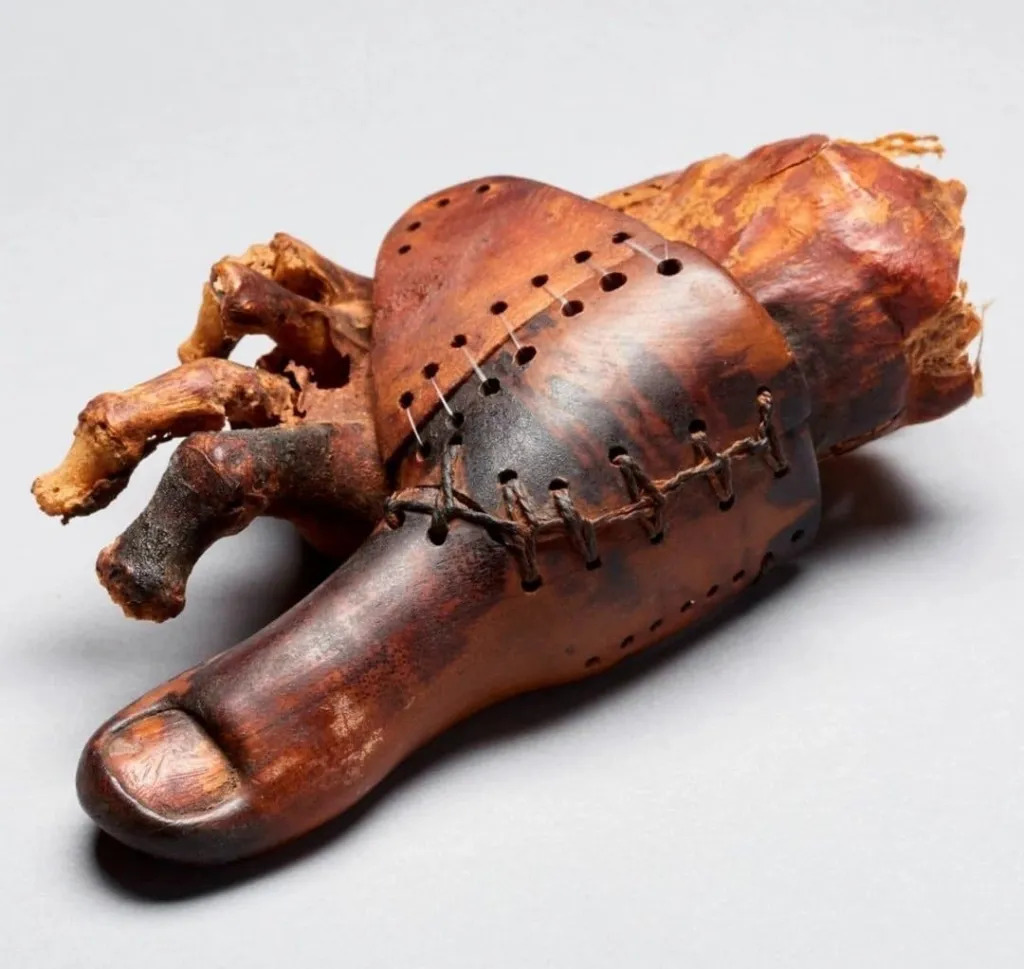
\includegraphics[width=0.4\textwidth]{figs/Egiptean.jpg}
	\caption{Proteză de deget din lemn și piele, descoperită la o mumie
	egipteană, una dintre cele mai vechi proteze cunoscute \cite{egiptmuseum}.}
	\label{fig:egiptean}
\end{figure}

Cele mai simple proteze, numite proteze pasive, nu au părți mobile și urmăresc în
principal refacerea aspectului estetic, oferind o funcționalitate de bază. Un pas
mai departe îl reprezintă protezele mecanice, acționate chiar de corpul
utilizatorului prin intermediul unui sistem de hamuri legat de mișcările umărului
sau ale cotului, iar această mișcare este transmisă mai departe printr-un cablu
către un cârlig sau o mână mecanică. Deși sunt dispozitive relativ simple, ele rămân și
astăzi printre cele mai răspândite proteze, tocmai datorită robusteții și a
costului redus \cite{hussein2014}.

\begin{figure}[H]
	\centering
	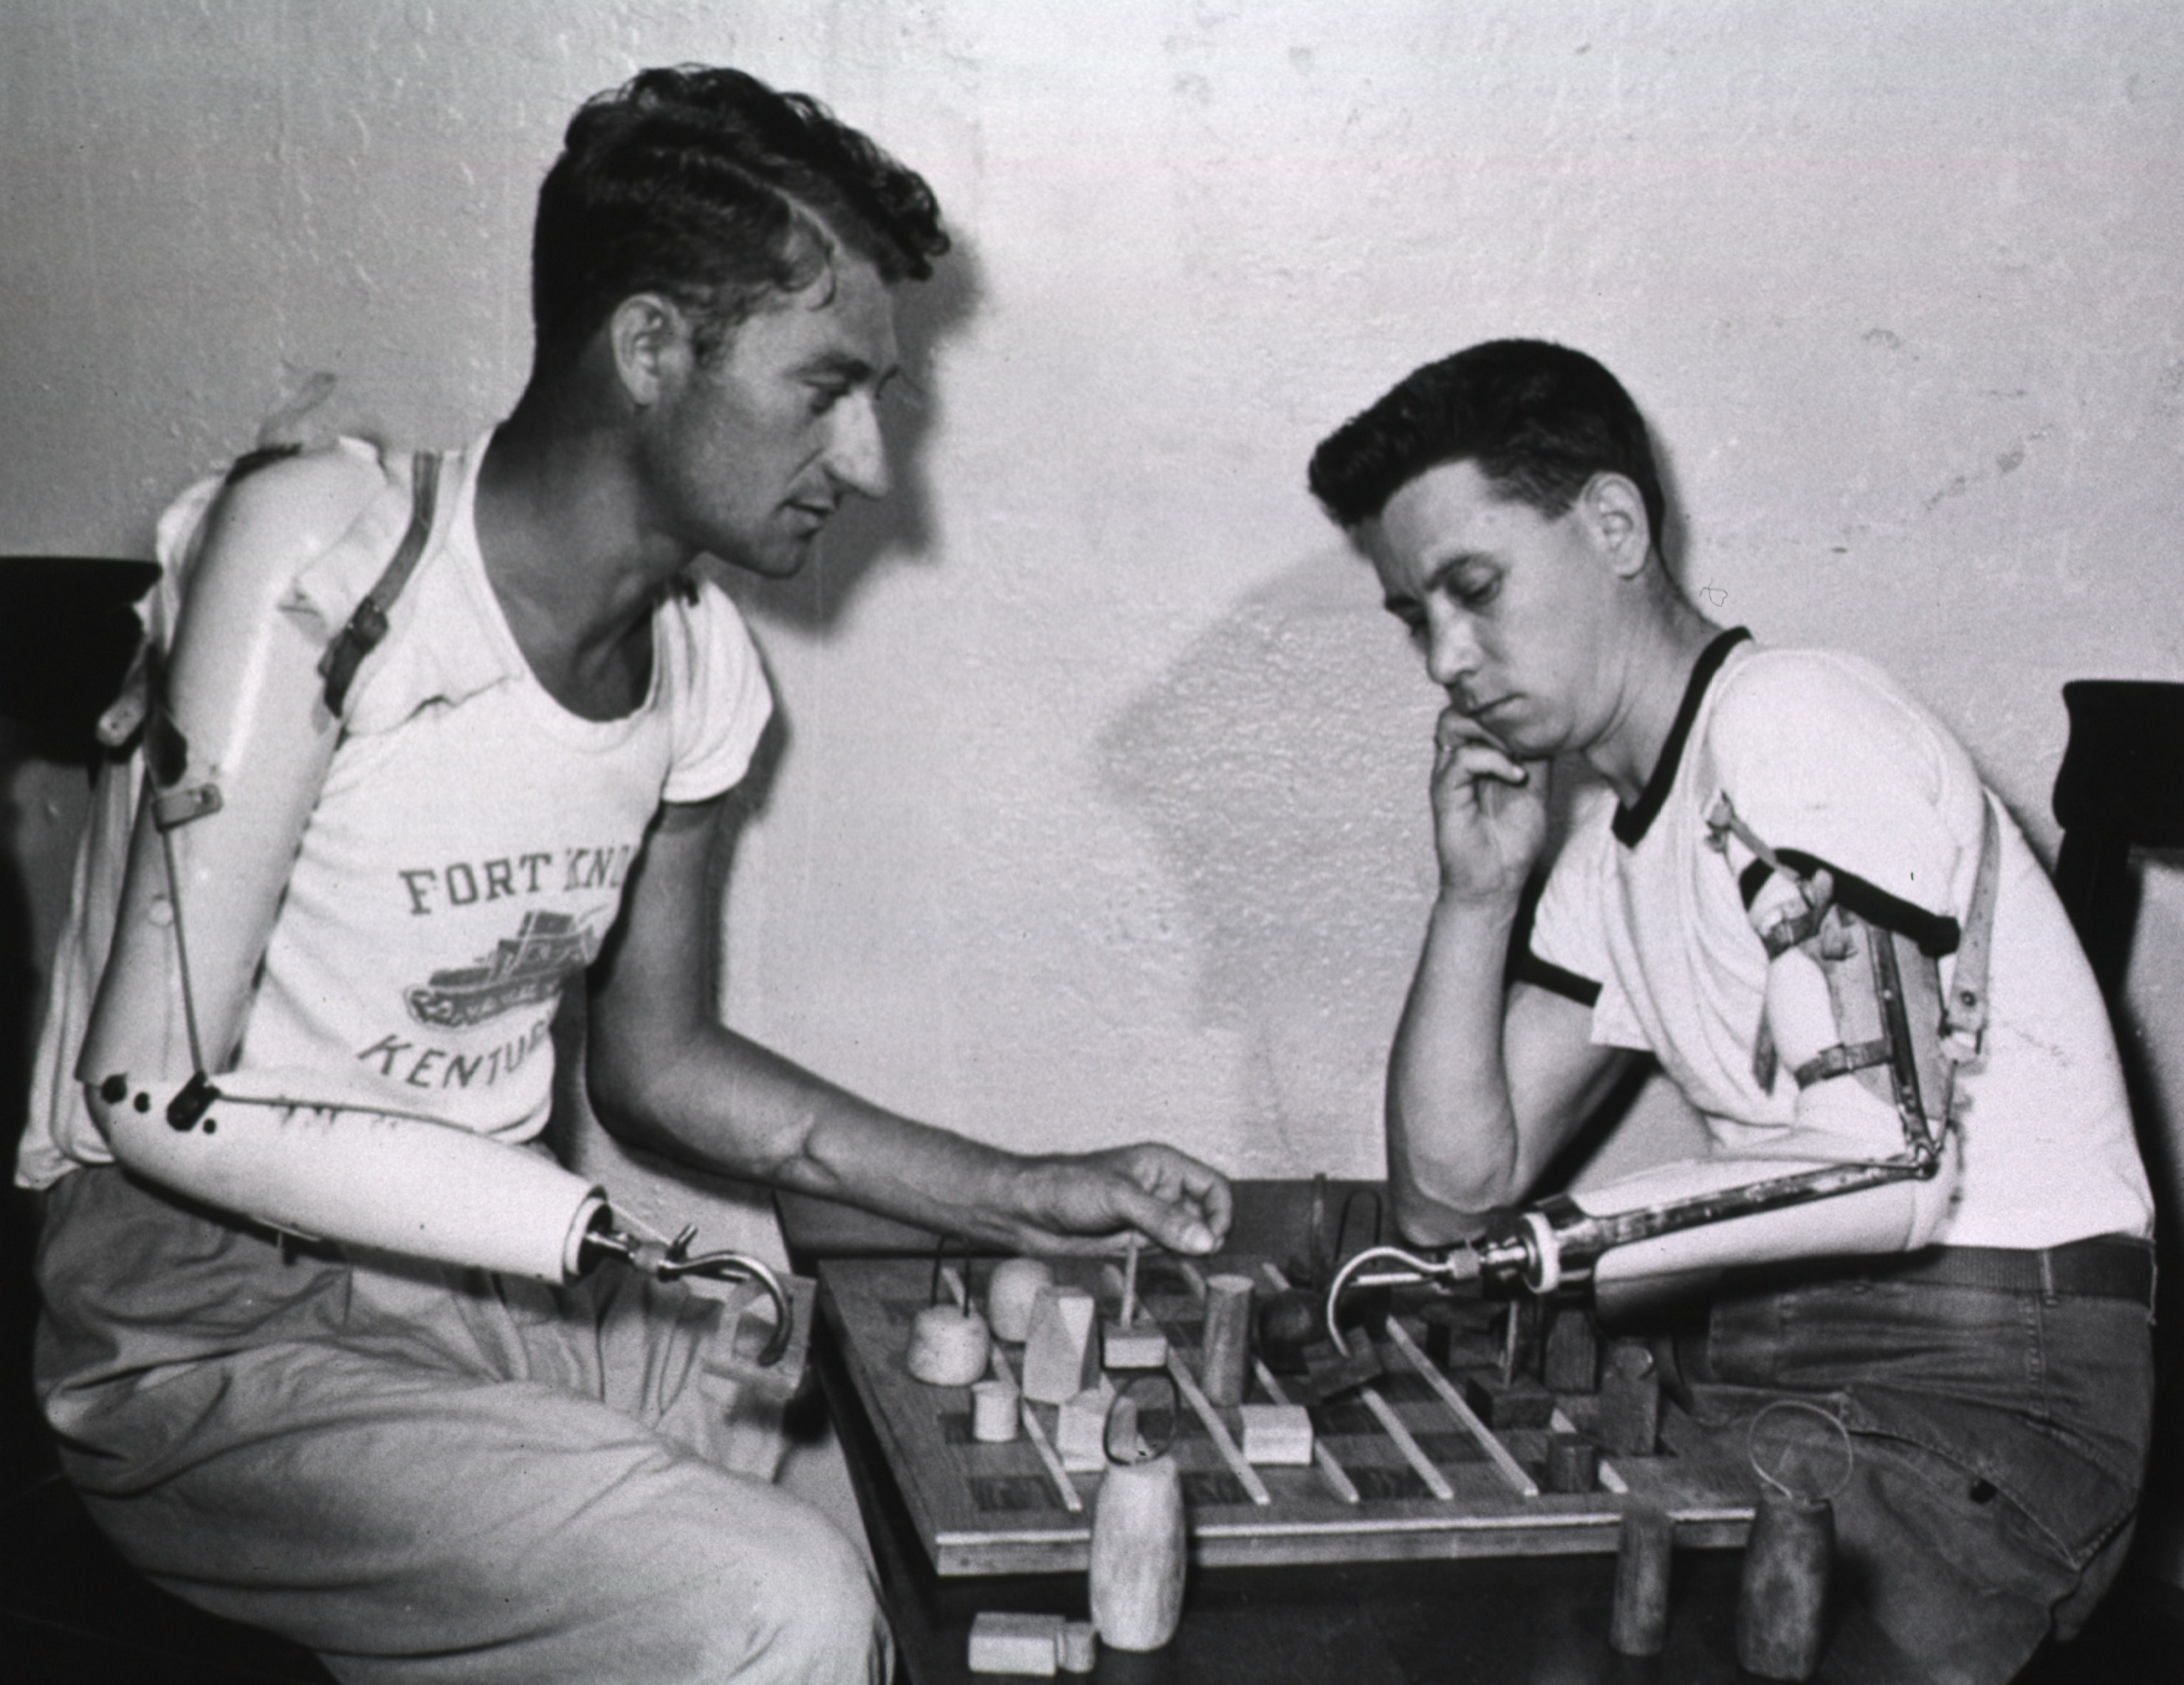
\includegraphics[width=0.45\textwidth]{figs/2Man.jpg}
	\caption{Proteze mecanice cu cârlig, acționate de corp prin hamuri și
	cabluri \cite{medlineplus}.}
	\label{fig:protezemecanice}
\end{figure}

Odată cu dezvoltarea electronicii a apărut o categorie mult mai performantă, aceea
a protezelor mioelectrice. Acestea funcționează măsurând semnalele electrice
produse de contracția mușchilor rămași în zona membrului afectat, semnale preluate
prin electrozi, amplificate și transmise unui microcontroler care comandă apoi
actuatoarele protezei. În acest fel, utilizatorul capătă un control mult mai fin
decât în cazul protezelor mecanice. La granița actuală a cercetării se află
interfețele neuronale directe, în care semnalele sunt preluate chiar de la nivelul
creierului prin electrozi implantați chirurgical. Deși o astfel de tehnologie este
încă la început, ea a demonstrat deja că o persoană poate comanda un braț robotic
doar prin gândire \cite{hussein2014}.

\begin{figure}[H]
	\centering
	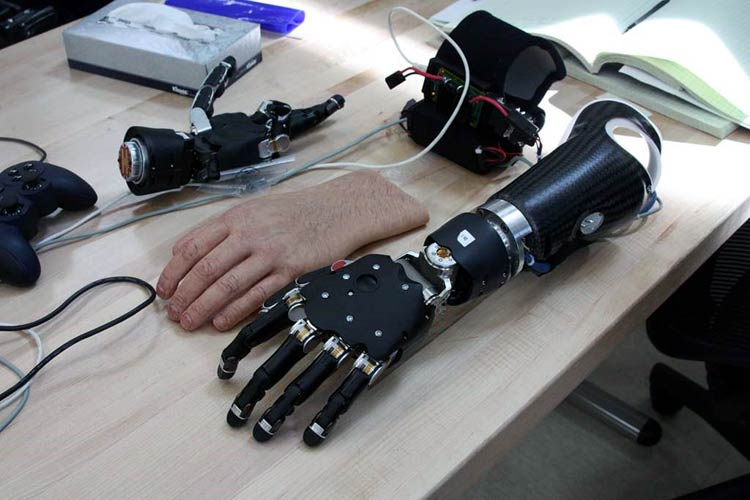
\includegraphics[width=0.5\textwidth]{figs/Modern1.jpg}
	\caption{Proteză modernă, acționată electronic, cu un grad ridicat de
	control asupra degetelor \cite{circuitdigest}.}
	\label{fig:protezamoderna}
\end{figure}

Sistemul realizat în această lucrare nu este o proteză mioelectrică în sensul
clasic, ci o mână robotică acționată în funcție de mișcările unei mâini umane
urmărite vizual. Cu toate acestea, el se bazează pe aceleași principii mecanice și
de control întâlnite la protezele moderne, iar înțelegerea acestora oferă contextul
necesar pentru restul lucrării.

\section{Anatomia mâinii și mâinile robotice biomimetice}
\label{sec:biblio-biomimetic}

Pentru a reproduce mișcările unei mâini este util să pornim de la complexitatea
modelului pe care încercăm să îl imităm. Mâna umană este alcătuită din cel puțin
27 de oase, peste 30 de mușchi și mai mult de o sută de ligamente, nervi și
artere, ceea ce o face un mecanism extrem de complex \cite{hussein2014}. Tocmai
de aceea, niciun sistem robotic actual nu reușește să egaleze dexteritatea și
fluiditatea unei mâini reale, iar orice proiect din acest domeniu pornește
inevitabil de la o variantă simplificată a ei.

\begin{figure}[H]
	\centering
	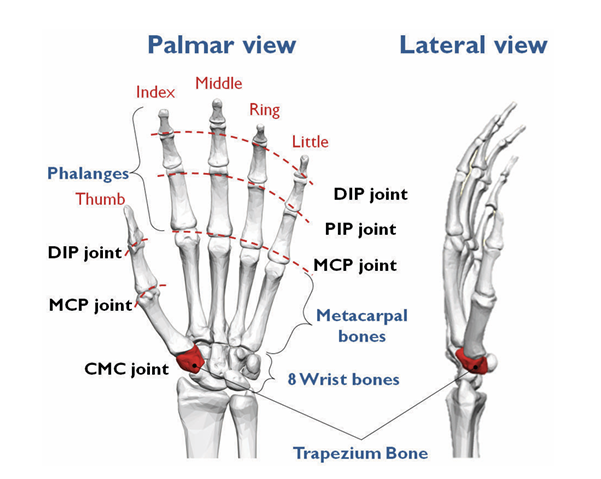
\includegraphics[width=0.55\textwidth]{figs/HumanHand.png}
	\caption{Structura osoasă a mâinii umane și articulațiile degetelor
	(DIP, PIP, MCP și CMC) \cite{biomimetic2016}.}
	\label{fig:anatomie}
\end{figure}

Un concept esențial pentru a descrie mișcarea unei astfel de structuri este cel de
grad de libertate (DOF), prin
care se înțelege o modalitate independentă în care un element se poate mișca. Un
deget uman, de pildă, dispune de patru grade de libertate. Trei dintre ele provin
din rotația articulațiilor sale și controlează împreună îndoirea și întinderea
degetului, iar al patrulea permite mișcarea laterală, de depărtare și apropiere
față de celelalte degete \cite{hussein2014}. Degetul mare beneficiază de un grad
suplimentar, ajungând astfel la cinci. Aceste mișcări sunt produse, în corpul
uman, prin contracția mușchilor și a tendoanelor, care trag de oase și le
deplasează.

\begin{figure}[H]
	\centering
	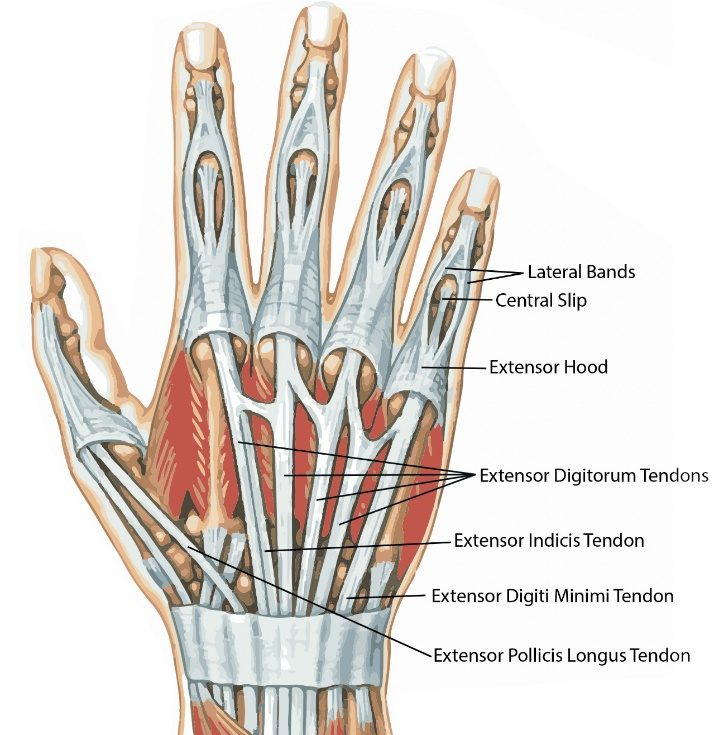
\includegraphics[width=0.4\textwidth]{figs/tendons.jpg}
	\caption{Rețeaua de tendoane extensoare de la nivelul mâinii, responsabilă
	de întinderea degetelor \cite{drgroh}.}
	\label{fig:tendoane}
\end{figure}

Mai exact, mișcarea degetelor este controlată de două grupe de tendoane care
acționează în sens opus. Tendoanele extensoare, situate pe partea dorsală a
mâinii, întind degetul, în timp ce tendoanele flexoare, de pe partea palmară,
îl îndoaie. Tendoanele flexoare sunt ghidate de-a lungul degetului prin niște
teci numite scripeți (\textit{pulleys}), care le mențin aproape de os și asigură
o îndoire controlată \cite{biomimetic2016}. Această pereche flexor-extensor este
exact principiul pe care îl reproduce un sistem robotic acționat prin tendoane.

\begin{figure}[H]
	\centering
	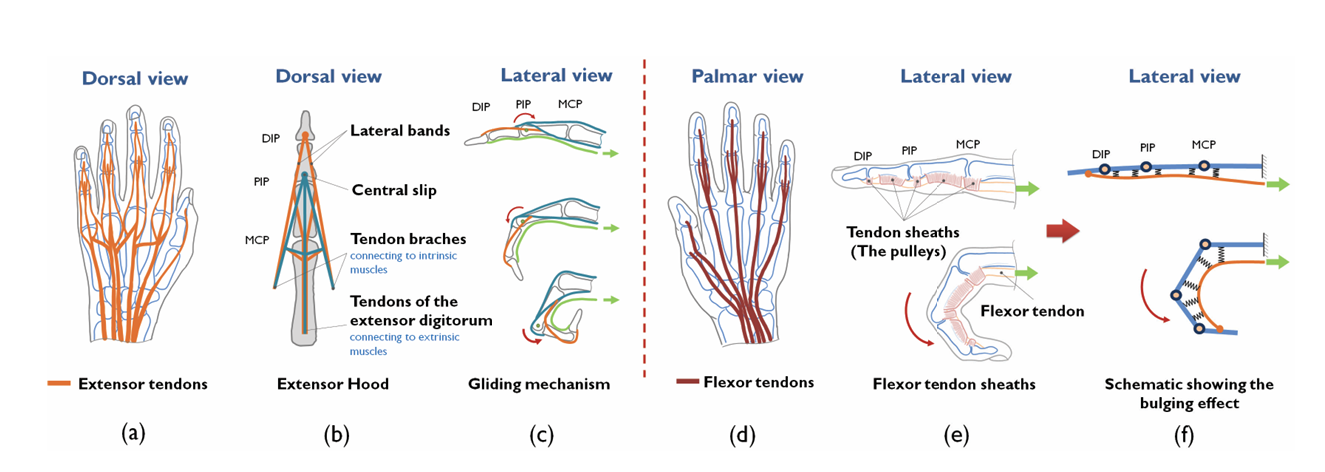
\includegraphics[width=0.95\textwidth]{figs/HumanHand2.png}
	\caption{Mecanismul tendoanelor la nivelul degetului: tendoanele extensoare
	(a--c) întind degetul, iar cele flexoare (d--f), ghidate prin scripeți,
	îl îndoaie \cite{biomimetic2016}.}
	\label{fig:flexorextensor}
\end{figure}

Acest mecanism natural a inspirat o întreagă categorie de mâini robotice, numite
biomimetice, care imită structura mâinii umane folosind tendoane artificiale ce
acționează degetele prin tragere, reproducând astfel îndoirea și întinderea lor
naturală \cite{biomimetic2016}. Atractivitatea acestei abordări vine din faptul că
oferă o metodă relativ simplă și ieftină de a controla degetele, fără a recurge la
mecanisme complicate.

Spre deosebire de aceasta, majoritatea protezelor comerciale folosesc un sistem de
articulații cuplate mecanic și acționate de motoare electrice \cite{hussein2014}.
Particularitatea lor este că toate articulațiile unui deget sunt comandate de un
singur motor, ceea ce înseamnă că întregul deget se poate mișca într-un singur mod,
deschizându-se și închizându-se la fel de fiecare dată. Practic, deși au tot atâtea
articulații ca un deget uman, aceste degete dispun de mult mai puține grade de
libertate, de obicei unul sau două față de cele patru ale degetului real. Această
limitare explică de ce protezele comerciale pot îndeplini doar sarcini relativ
simple și nu pot reproduce varietatea de gesturi pe care le permite o mână
adevărată.

Există însă și lucrări de cercetare care urmăresc apropierea cât mai mare de modelul
biologic. Una dintre ele propune o mână robotică antropomorfă cu un grad ridicat de
biomimetism, care reproduce fidel structura și mișcările mâinii umane
\cite{biomimetic2016}. Un astfel de proiect a constituit o sursă de inspirație
pentru conceptele preluate în lucrarea de față, în special pentru modul în care
mișcările sunt distribuite pe articulații. Reproducerea integrală a unei asemenea
structuri presupune însă costuri ridicate și o complexitate mecanică greu de atins
în cadrul unui proiect de licență, motiv pentru care soluția aleasă aici pornește
de la o variantă mai simplă, construită din componente accesibile.

\section{Proiecte open-source de mâini robotice}
\label{sec:biblio-opensource}

Dincolo de cercetarea academică și de produsele comerciale, în ultimii ani s-a
dezvoltat o comunitate amplă de proiecte open-source dedicate mâinilor și brațelor
robotice. Acestea pun la dispoziție gratuit modele tridimensionale care pot fi
printate 3D și asamblate de oricine, fiind însoțite de obicei de o documentație
extinsă și de o comunitate activă de pasionați. Pentru proiectul de față, aceste
resurse au reprezentat punctul de plecare, fiecare contribuind cu o parte din
ansamblul final. În continuare sunt prezentate proiectele studiate și ceea ce a
fost preluat din fiecare.

\subsection{InMoov}
\label{sec:biblio-inmoov}

Cel mai cunoscut proiect open-source din acest domeniu este InMoov, primul robot
umanoid de dimensiune reală conceput pentru a fi în întregime printat 3D
\cite{inmoov2014}. Datorită documentației extinse și a comunității active care
s-a format în jurul său, InMoov a devenit un punct de referință pentru proiectele
de mâini robotice accesibile. Mâna sa utilizează aproximativ șase servomotoare și
acționează degetele prin tendoane, fiecare deget fiind tras de un cablu.

\begin{figure}[H]
	\centering
	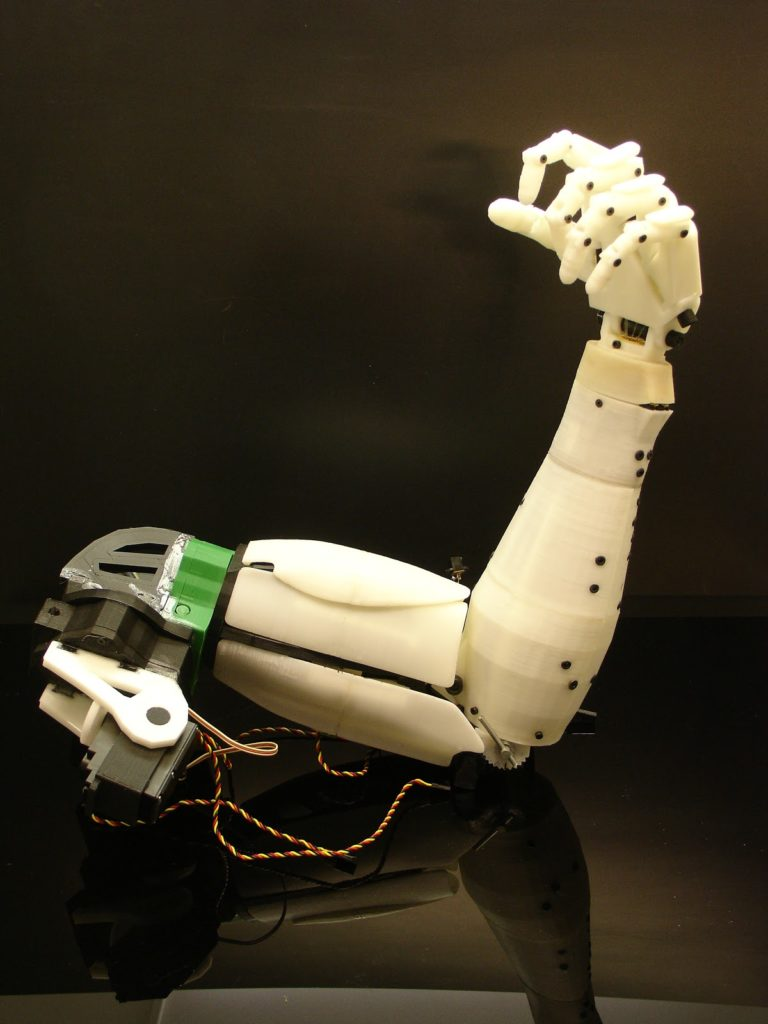
\includegraphics[width=0.5\textwidth]{figs/inmoovArm.jpg}
	\caption{Brațul robotic InMoov, printat 3D \cite{inmoov2014}.}
	\label{fig:inmoovarm}
\end{figure}

Din acest proiect am preluat soluția pentru rotația încheieturii, care mi s-a părut
cea mai bine gândită din punctul de vedere al ghidării firelor. Sistemul de
scripeți care rotesc mâna s-a dovedit deosebit de util și ușor de integrat în
restul ansamblului, motiv pentru care l-am păstrat aproape neschimbat.

\begin{figure}[H]
	\centering
	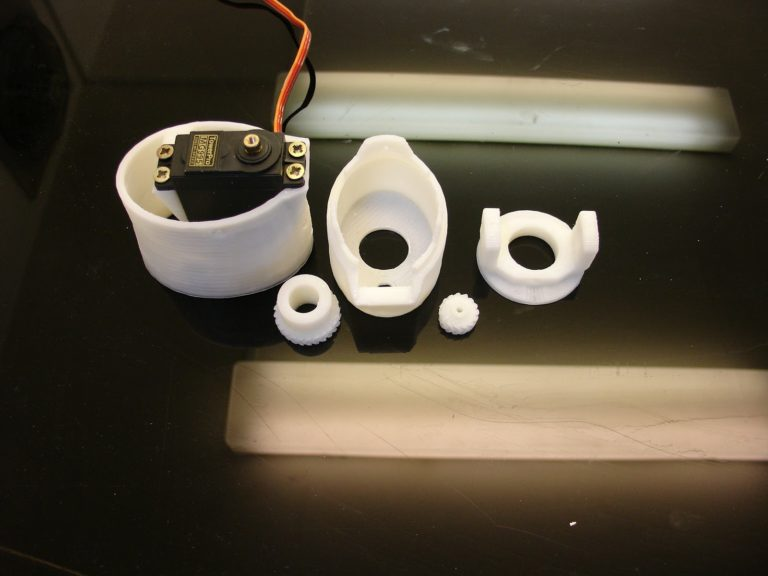
\includegraphics[width=0.55\textwidth]{figs/inmoovWrist.jpg}
	\caption{Mecanismul de rotație a încheieturii din proiectul InMoov, format
	dintr-un servomotor și componente printate 3D \cite{inmoov2014}.}
	\label{fig:inmoovwrist}
\end{figure}

\subsection{Modelul palmei}
\label{sec:biblio-ryonicle}

Palma și degetele propriu-zise au fost preluate de la un model dezvoltat de
Ryonicle, disponibil public pe platforma Thingiverse \cite{ryonicle}. Acest model
mi-a atras atenția prin forma sa îngrijită și prin modul de acționare a degetelor:
fiecare deget este tras de un servomotor prin intermediul unui tendon, iar
revenirea în poziția inițială se face cu ajutorul unor elastice care joacă rolul
tendoanelor extensoare. Această soluție reproduce, într-o formă simplificată,
perechea flexor-extensor întâlnită la mâna umană.

\begin{figure}[H]
	\centering
	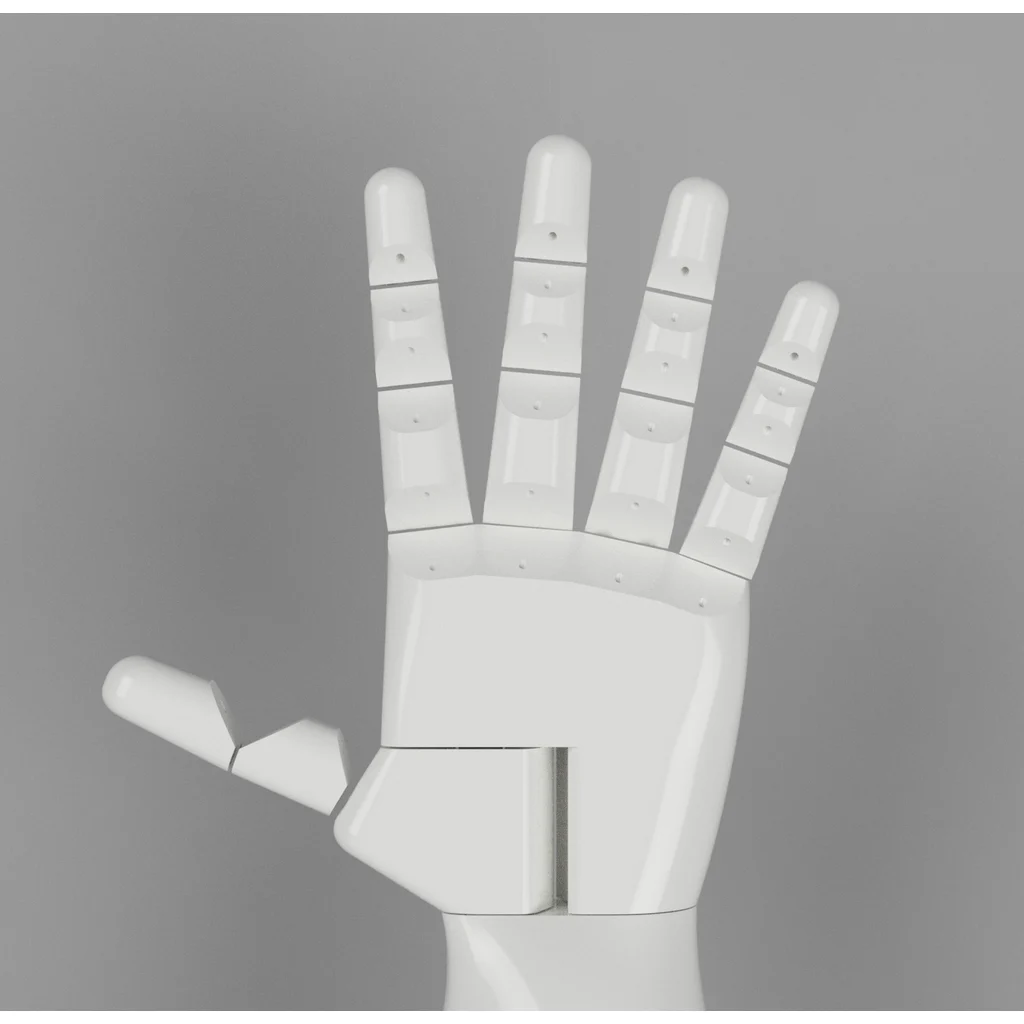
\includegraphics[width=0.45\textwidth]{figs/ryonicleHand.png}
	\caption{Modelul de mână dezvoltat de Ryonicle, de la care au fost preluate
	palma și degetele \cite{ryonicle}.}
	\label{fig:ryonicle}
\end{figure}

Modelul original folosea însă un alt tip de servomotoare decât cele alese în
proiectul de față, ceea ce a impus câteva adaptări la nivelul locașurilor și al
modului de prindere.

\subsection{Antebrațul și cotul}
\label{sec:biblio-hussein}

Pentru zona de la încheietură în jos, mai exact întreg antebrațul și articulația
cotului, împreună cu sistemul de scripeți aferent, am pornit de la modelul propus
de Mahdi Hussein în teza sa dedicată unui braț protetic printat 3D
\cite{hussein2014}. Această parte găzduiește servomotoarele care acționează
degetele și asigură traseul tendoanelor către mână, integrându-se bine cu restul
ansamblului.

\begin{figure}[H]
	\centering
	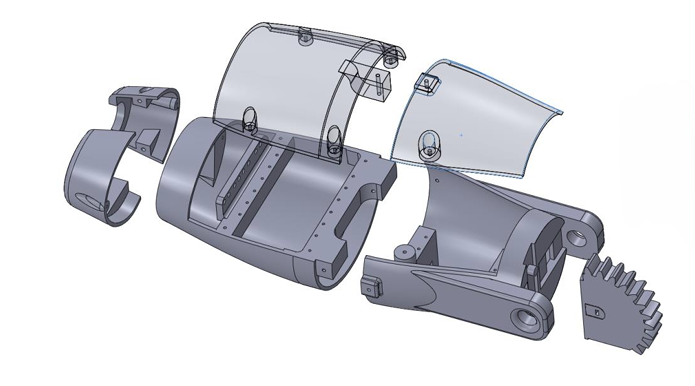
\includegraphics[width=0.6\textwidth]{figs/husseinForearm.png}
	\caption{Modelul antebrațului propus de Hussein, preluat pentru zona de la
	încheietură în jos \cite{hussein2014}.}
	\label{fig:husseinforearm}
\end{figure}

\subsection{Horizon}
\label{sec:biblio-horizon}

Un alt proiect avut în vedere a fost cel prezentat de Horizon \cite{horizon_hand}.
Deși am purtat o corespondență cu autorul pentru a obține fișierele necesare,
modelul său de mână, de tip osos, nu se potrivea cu obiectivul meu de a realiza un
braț aproape complet, fără umăr. Combinarea lui cu celelalte componente s-ar fi
făcut cu dificultate, iar stabilitatea mișcărilor ar fi avut de suferit. În plus,
cadrul propus de el era de dimensiuni mari și greu de adaptat la restul
ansamblului, motiv pentru care, în final, nu a fost folosit.

Aceste proiecte au constituit baza de la care a pornit soluția proprie, un ansamblu
hibrid ce preia de la fiecare sursă partea cea mai potrivită, iar modul concret în
care au fost combinate este detaliat în capitolul de proiectare și implementare.

\section{Filtrul Kalman}
\label{sec:biblio-kalman}

Componenta centrală a lucrării de față, cea care prelucrează datele de mișcare
înainte de a fi trimise spre servomotoare, este un filtru Kalman. Acesta este un
algoritm de estimare propus de Rudolf Kalman în anul 1960 \cite{kalman1960} și a
devenit, de atunci, unul dintre cele mai utilizate instrumente pentru estimarea
stării unui sistem dinamic afectat de zgomot. El este folosit pe scară largă în
domenii precum navigația, robotica sau procesarea semnalelor, oriunde este nevoie
de o estimare cât mai exactă a unei mărimi pornind de la măsurători imperfecte.

Ideea de bază a filtrului este aceea de a combina două surse de informație, fiecare
imperfectă în felul ei. Pe de o parte există o predicție, obținută pe baza unui
model matematic al sistemului, care spune cum ar trebui să evolueze starea în timp.
Pe de altă parte există o măsurătoare reală, dar afectată de zgomot. Filtrul
cântărește aceste două surse în funcție de cât de mult se poate avea încredere în
fiecare și produce o estimare finală mai bună decât oricare dintre ele luată
separat. Rezultatul este o valoare netezită, care urmărește fidel evoluția reală a
sistemului, eliminând în același timp variațiile bruște cauzate de zgomot.

Din punct de vedere matematic, sistemul este descris printr-un vector de stare
$\mathbf{x}$, care reține mărimile estimate, și printr-o matrice de covarianță
$\mathbf{P}$, care exprimă incertitudinea asociată acestor estimări. Algoritmul
funcționează ciclic, alternând două etape. În etapa de predicție, starea și
incertitudinea sunt proiectate înainte în timp pe baza modelului sistemului,
descris de matricea de tranziție $\mathbf{F}$ și de zgomotul de proces
$\mathbf{Q}$ \cite{welch1995}:
%
\begin{align}
	\hat{\mathbf{x}}_{k}^{-} &= \mathbf{F}\,\hat{\mathbf{x}}_{k-1} \\
	\mathbf{P}_{k}^{-} &= \mathbf{F}\,\mathbf{P}_{k-1}\,\mathbf{F}^{\top} + \mathbf{Q}
\end{align}
%
În etapa de actualizare, predicția este corectată cu ajutorul măsurătorii
$\mathbf{z}_k$. Se calculează mai întâi câștigul Kalman $\mathbf{K}_k$, care
stabilește cât de mult se ține cont de măsurătoare față de predicție, după care
starea și covarianța sunt corectate \cite{welch1995}:
%
\begin{align}
	\mathbf{K}_k &= \mathbf{P}_{k}^{-}\mathbf{H}^{\top}
	\left(\mathbf{H}\,\mathbf{P}_{k}^{-}\mathbf{H}^{\top} + \mathbf{R}\right)^{-1} \\
	\hat{\mathbf{x}}_{k} &= \hat{\mathbf{x}}_{k}^{-}
	+ \mathbf{K}_k\left(\mathbf{z}_k - \mathbf{H}\,\hat{\mathbf{x}}_{k}^{-}\right) \\
	\mathbf{P}_{k} &= \left(\mathbf{I} - \mathbf{K}_k\,\mathbf{H}\right)\mathbf{P}_{k}^{-}
\end{align}
%
Aici $\mathbf{H}$ este matricea de observație, care leagă starea de mărimea
măsurată, $\mathbf{R}$ reprezintă zgomotul de măsurare, iar $\mathbf{I}$ este
matricea identitate. Diferența $\mathbf{z}_k - \mathbf{H}\,\hat{\mathbf{x}}_{k}^{-}$,
numită inovație, arată cât de mult se abate măsurătoarea de la predicție, iar
câștigul Kalman decide proporția în care această abatere corectează estimarea.

Pentru documentarea pe acest subiect, înțelegerea intuitivă a algoritmului a fost
facilitată de prezentarea accesibilă realizată de Alan Zucconi \cite{zucconi2022},
în timp ce fundamentele teoretice riguroase au fost aprofundate pe baza lucrărilor
clasice din domeniu \cite{welch1995}. Modul concret în care filtrul a fost adaptat
și implementat în cadrul acestui proiect este detaliat în capitolul de analiză și
fundamentare teoretică.

\section{Servomotoare și controlul prin PWM}
\label{sec:biblio-servo}

Mișcarea efectivă a degetelor și a articulațiilor brațului robotic este realizată
de servomotoare. Un servomotor este un actuator format dintr-un motor electric,
un sistem de angrenaje și un circuit intern de control, care îi permite să se
deplaseze într-o poziție unghiulară dorită și să o mențină. Spre deosebire de un
motor obișnuit, care se rotește continuu, servomotorul primește o comandă de
poziție și se deplasează exact în punctul indicat, ceea ce îl face potrivit pentru
controlul articulațiilor unei mâini robotice.

Comanda de poziție se transmite printr-un semnal de tip PWM. Acesta este un semnal
periodic la care
nu amplitudinea, ci durata pulsului activ codifică informația. În cazul
servomotoarelor uzuale, semnalul are o perioadă de 20 de milisecunde, iar durata
pulsului variază în general între 1 și 2 milisecunde. Un puls scurt corespunde unei
poziții la o extremă a cursei, un puls lung corespunde celeilalte extreme, iar
valorile intermediare determină proporțional unghiul dorit. Circuitul intern al
servomotorului compară permanent poziția curentă cu cea comandată și acționează
motorul până când cele două coincid.

Pentru acest proiect a fost ales servomotorul MG996R, un model larg răspândit, cu
angrenaje metalice și un cuplu de aproximativ 11~kg$\cdot$cm \cite{mg996r_datasheet}.
Alegerea s-a bazat în principal pe cuplul ridicat, necesar pentru a trage de
tendoanele care acționează degetele și pentru a învinge rezistența elementelor
elastice de revenire. Caracteristicile detaliate ale acestui servomotor, precum și
modul în care sunt generate semnalele PWM în cadrul sistemului, sunt prezentate în
capitolele următoare.

\section{Fabricarea prin printare 3D}
\label{sec:biblio-print3d}

Componentele mecanice ale brațului robotic sunt realizate prin printare 3D, o
tehnologie de fabricație aditivă în care obiectul este construit strat cu strat,
pornind de la un model tridimensional. Cea mai răspândită variantă, folosită și în
acest proiect, este depunerea de material topit (FDM, \textit{Fused Deposition
Modeling}), în care un filament de material plastic este încălzit și depus succesiv
de o duză care se deplasează după contururile fiecărui strat. Această metodă a
devenit accesibilă și ieftină, permițând realizarea unor piese complexe într-un
timp relativ scurt, motiv pentru care este preferată în majoritatea proiectelor de
mâini robotice open-source.

Alegerea materialului are un rol important asupra rezistenței și durabilității
pieselor. Cel mai utilizat filament este PLA (\textit{Polylactic Acid}), apreciat
pentru ușurința la printare, însă relativ casant și sensibil la temperatură. O
alternativă mai rezistentă este ABS (\textit{Acrylonitrile Butadiene Styrene}),
mai dur, dar mai dificil de printat și predispus la deformări. Pentru acest
proiect a fost ales PETG (\textit{Polyethylene Terephthalate Glycol}), care
combină avantajele celor două, oferind o rezistență mecanică și o flexibilitate
superioare PLA-ului, fără dificultățile de printare ale ABS-ului. Această
rezistență este esențială pentru piesele unei mâini robotice, care sunt supuse în
mod constant la tensiunile produse de tendoane și de elementele elastice.

Pe lângă alegerea materialului, calitatea pieselor depinde și de parametrii de
printare, precum densitatea de umplere, numărul de straturi exterioare sau
înălțimea unui strat. Documentarea privind aceste setări și ajustarea lor pentru
piesele brațului robotic au necesitat mai multe încercări, fabricarea completă a
componentelor însumând aproximativ 32 de ore de printare.
